%% Template for MLP Coursework 1 / 12 October 2026

%% Based on  LaTeX template for ICML 2017 - example_paper.tex at 
%%  https://2017.icml.cc/Conferences/2017/StyleAuthorInstructions

\documentclass{article}
\usepackage[T1]{fontenc}
\usepackage{amssymb,amsmath}
\usepackage{txfonts}
\usepackage{microtype}

% For figures
\usepackage{graphicx}
\usepackage{subcaption} 

% For citations
\usepackage{natbib}

% For algorithms
\usepackage{algorithm}
\usepackage{algorithmic}

% the hyperref package is used to produce hyperlinks in the
% resulting PDF.  If this breaks your system, please commend out the
% following usepackage line and replace \usepackage{mlp2017} with
% \usepackage[nohyperref]{mlp2017} below.
\usepackage{hyperref}
\usepackage{url}
\urlstyle{same}

\usepackage{color}
\usepackage{booktabs} % To thicken table lines
\usepackage{multirow} % Multirow cells in table
\usepackage{soul}
\usepackage{bm}

% Packages hyperref and algorithmic misbehave sometimes.  We can fix
% this with the following command.
% \newcommand{\theHalgorithm}{\arabic{algorithm}}


% Set up MLP coursework style (based on ICML style)
\usepackage{mlp2022}
\mlptitlerunning{MLP 2026/27: Coursework 1 (\studentNumber)}
\bibliographystyle{icml2017}


\DeclareMathOperator{\softmax}{softmax}
\DeclareMathOperator{\sigmoid}{sigmoid}
\DeclareMathOperator{\sgn}{sgn}
\DeclareMathOperator{\relu}{relu}
\DeclareMathOperator{\lrelu}{lrelu}
\DeclareMathOperator{\elu}{elu}
\DeclareMathOperator{\selu}{selu}
\DeclareMathOperator{\maxout}{maxout}



\definecolor{red}{rgb}{0.95,0.4,0.4}
\definecolor{blue}{rgb}{0.4,0.4,0.95}
\definecolor{orange}{rgb}{1, 0.65, 0}

\newcommand{\youranswer}[1]{{\color{red} \bf[#1]}} %your answer: 


%% START of YOUR ANSWERS
%% REPLACE SXXXXXX with your student number
\def\studentNumber{SXXXXXX}


%% START of YOUR ANSWERS
%% Add answers to the questions below, by replacing the text inside the brackets {} for \youranswer{ "Text to be replaced with your answer." }. 
%
% Do not delete the commands for adding figures and tables. Instead fill in the missing values with your experiment results, and replace the images with your own respective figures.
%
% You can generally delete the placeholder text, such as for example the text "Question Figure 2 - Replace the images ..." 
%
% There are 6 TEXT QUESTIONS. Replace the text inside the brackets of the command \youranswer with your answer to the question.
%
% There are also 2 "questions" to replace or add FIGURES, and 2 "questions" asking you to fill in missing TABLE entries or add a TABLE. The figures and tables in the problem identification section are provided.
%
% NOTE! that questions are ordered by the order of appearance of their answers in the text, and not by the order you should tackle them. You should complete the relevant experiments and fill in the TABLES and FIGURES before discussing the results presented there.
%
% NOTE! If for some reason you do not manage to produce results for some FIGURES and TABLES, then you can get partial marks by discussing your expectations of the results in the relevant TEXT QUESTIONS (for example Question 2 makes use of Table 3 and Figure 4).
%
% Please refer to the coursework specification for more details.


%% - - - - - - - - - - - - TEXT QUESTIONS - - - - - - - - - - - - 



%% Question 1:
\newcommand{\questionOne} {
\youranswer{Question 1 - Find and read the paper by Zou and Hastie (2005) specified in the coursework description. Explain na\"ive elastic net and its potential benefits. Cite the paper and provide relevant equations, considering both training and inference, explaining all variables and hyperparameters. Describe how you will implement this approach in PyTorch for the experiments in the next section.}
}

%% Question 2:
\newcommand{\questionTwo} {
\youranswer{Question 2 - Analyse and explain the results in Table~3 and Figure~4 on testing each regularization technique separately. While discussing na\"ive elastic net, mention how you decided on the hyperparameter values for it.
}
}

%% Question 3:
\newcommand{\questionThree} {
\youranswer{Question 3 - Using the supplied results and your experiments in Table~3, select and justify exactly \textbf{10} additional configurations varying the regularisation techniques and their hyperparameters. Select and justify all ten configurations before running them; sequential selection based on their results is not permitted. Follow the common experimental settings specified in the coursework description. These ten runs exclude the five runs needed to complete Table~3, the independent-method experiment in Question~5, and any necessary retraining for test evaluation. Run the ten experiments and present their results in Table~4 and Figure~5. You are assessed on your justification, correct experimental setup and execution, and analysis of the results, rather than on achieving high performance. Discuss the results in Question~4.}
}


%% Question 4:
\newcommand{\questionFour} {
\youranswer{Question 4 - Explain the experimental settings, including hyperparameters, and analyse the results in Tables~3 and~4 and Figures~4 and~5 in terms of generalisation performance and overfitting. Report epoch-100 results. Report ordinary cross-entropy against the original, unsmoothed labels, excluding all weight penalties. Follow the supplied notebook's convention for measuring training error and state that convention. Select the best configuration from Tables~3 and~4 using epoch-100 validation accuracy, using validation cross-entropy to break ties. Evaluate the selected model on the test set only after completing this selection, and report and discuss its test performance.}
}


%% Question 5:
\newcommand{\questionFive} {
\youranswer{Question 5 - Independently identify a regularisation approach other than dropout, L1, L2, na\"ive elastic net or label smoothing. Find and cite a research paper describing the approach. Explain its mechanism, relevant hyperparameters, and why it may help address overfitting in this task. Implement the approach in PyTorch and run one additional EMNIST experiment consisting of a single training run. Explain your implementation and justify your hyperparameter choices. Use the common architecture and training settings wherever compatible with the approach, explaining any necessary departures. Report validation accuracy, training and validation cross-entropy, and the generalisation gap, following the reporting conventions in the specification. Compare its validation results with those of the configuration selected in Question~4. Explain any differences in experimental settings that affect this comparison, and discuss the approach's benefits and limitations, recognising the limited evidence from one run. This experiment is additional to the ten runs required for Question~3.}
}

%% Question 6:
\newcommand{\questionSix} {
\youranswer{Question 6 - Briefly draw your conclusions based on the results from the previous sections (what are the take-away messages?), discussing them in the context of the overall literature, and conclude your report with a recommendation for future directions.}
}

%% - - - - - - - - - - - - FIGURES - - - - - - - - - - - - 

%% Question Figure 2:
\newcommand{\questionFigureTwo} {
    \begin{figure}[t]
        \centering
        \begin{subfigure}{\linewidth}
            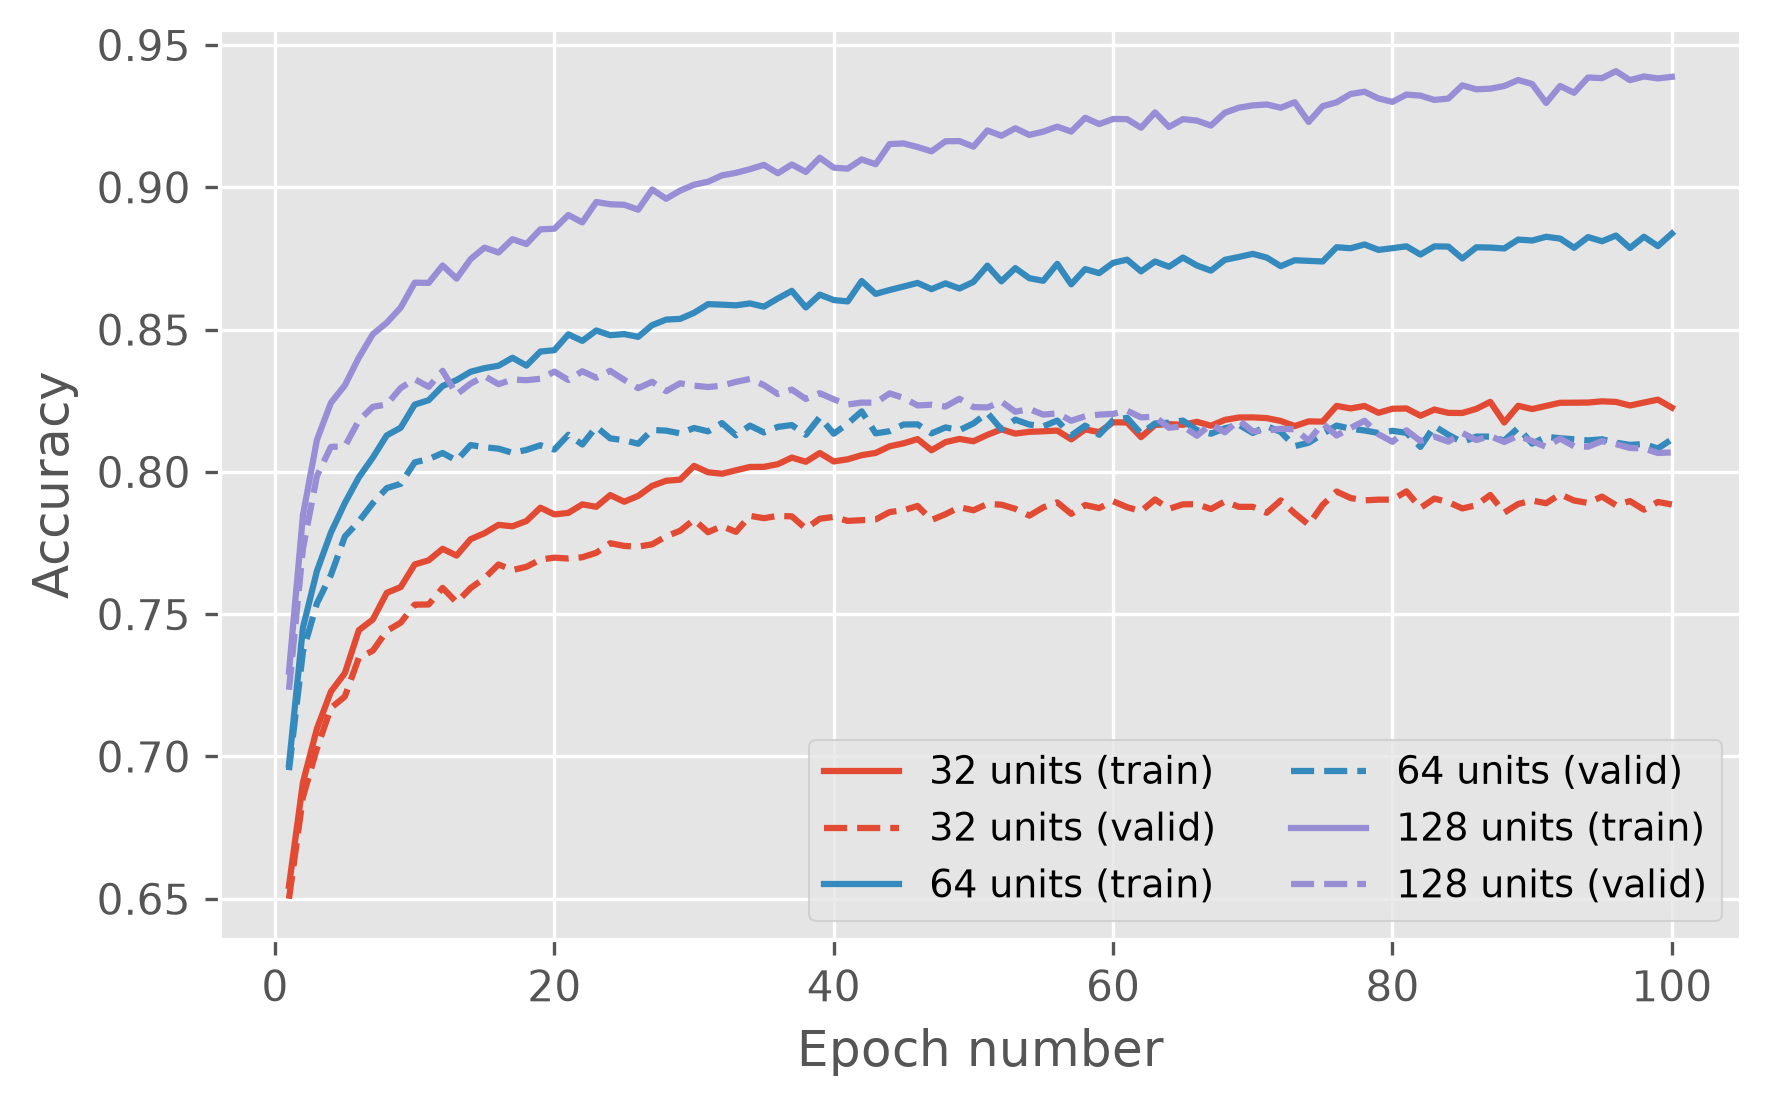
\includegraphics[width=\linewidth]{figures/fig2_width_accuracy.png}
            \caption{Accuracy by epoch.}
            \label{fig:width_acccurves}
        \end{subfigure}
        \begin{subfigure}{\linewidth}
            \centering
            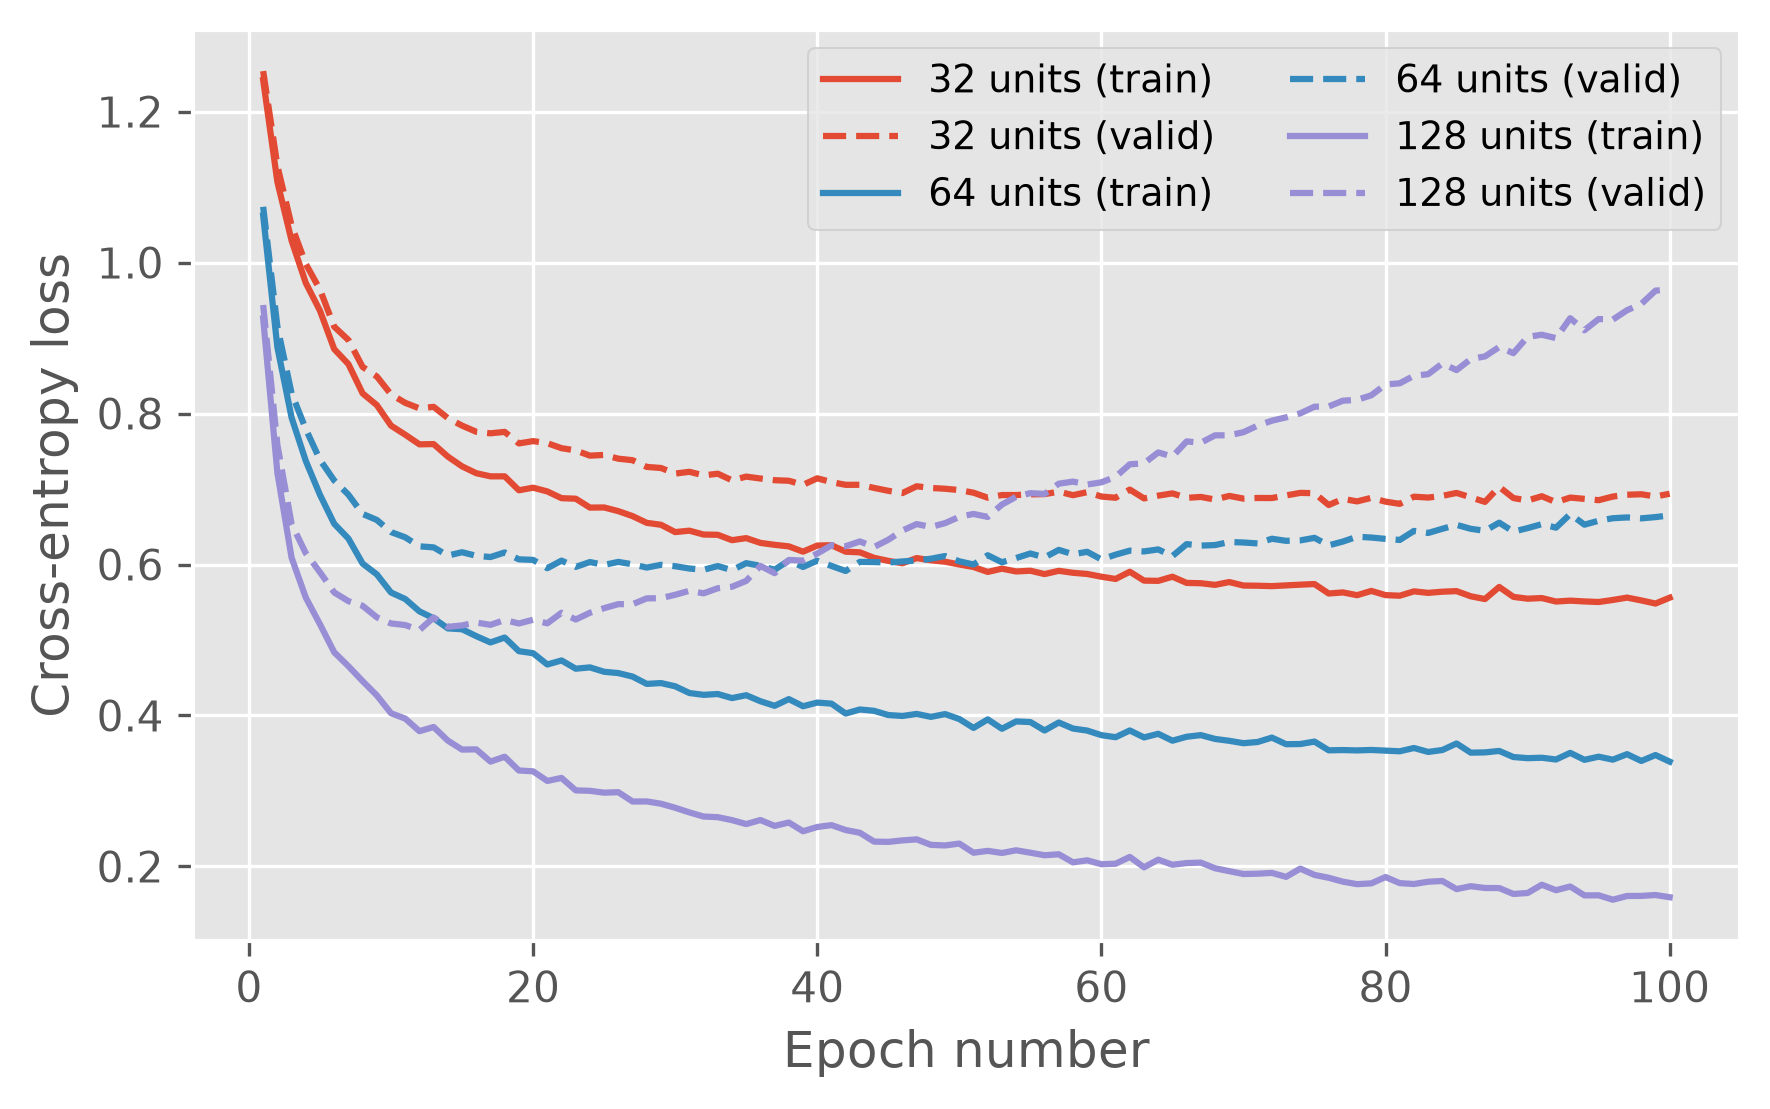
\includegraphics[width=\linewidth]{figures/fig2_width_loss.png}
            \caption{Cross-entropy by epoch.}
            \label{fig:width_errorcurves}
        \end{subfigure}
        \caption{Training (solid) and validation (dashed) accuracy and cross-entropy over 100 epochs for one-hidden-layer networks with 32, 64, or 128 ReLU units. }
        \label{fig:width}
    \end{figure}
}

%% Question Figure 3:
\newcommand{\questionFigureThree} {
    \begin{figure}[t]
        \centering
        \begin{subfigure}{\linewidth}
            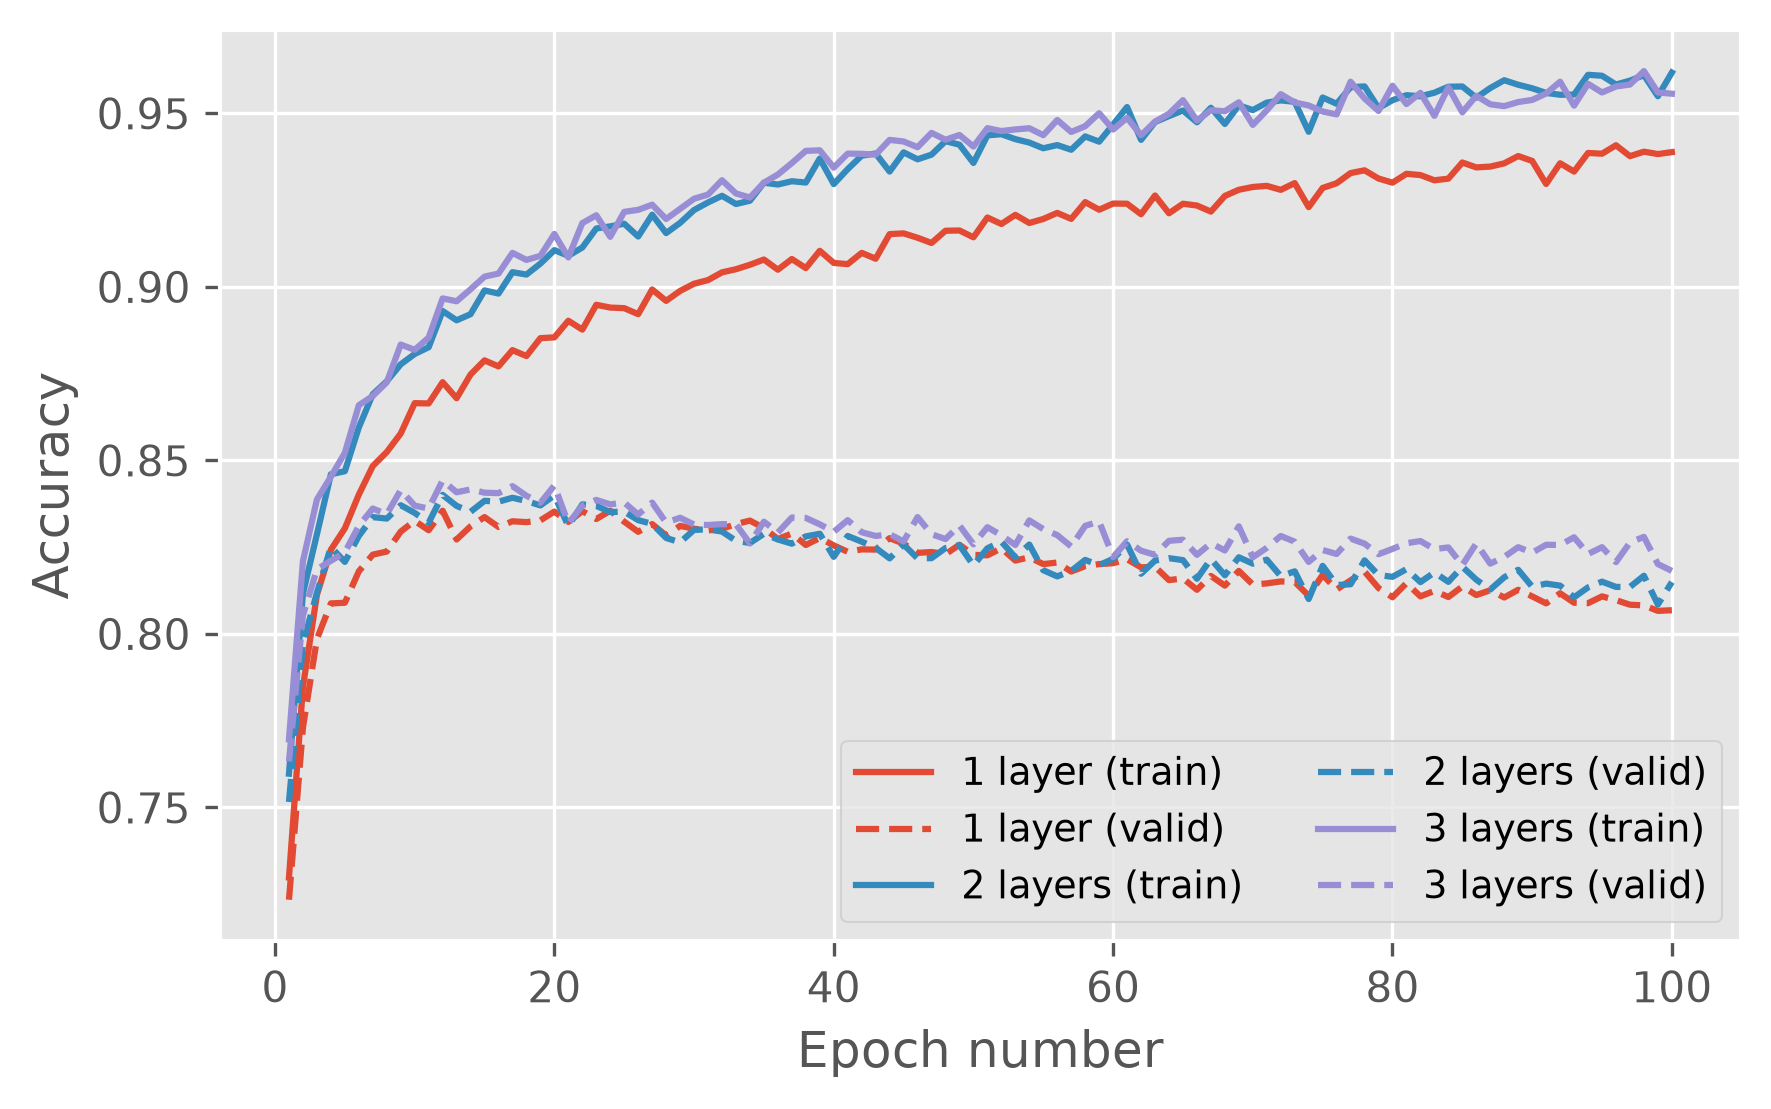
\includegraphics[width=\linewidth]{figures/fig3_depth_accuracy.png}
            \caption{Accuracy by epoch.}
            \label{fig:depth_acccurves}
        \end{subfigure}
        \begin{subfigure}{\linewidth}
            \centering
            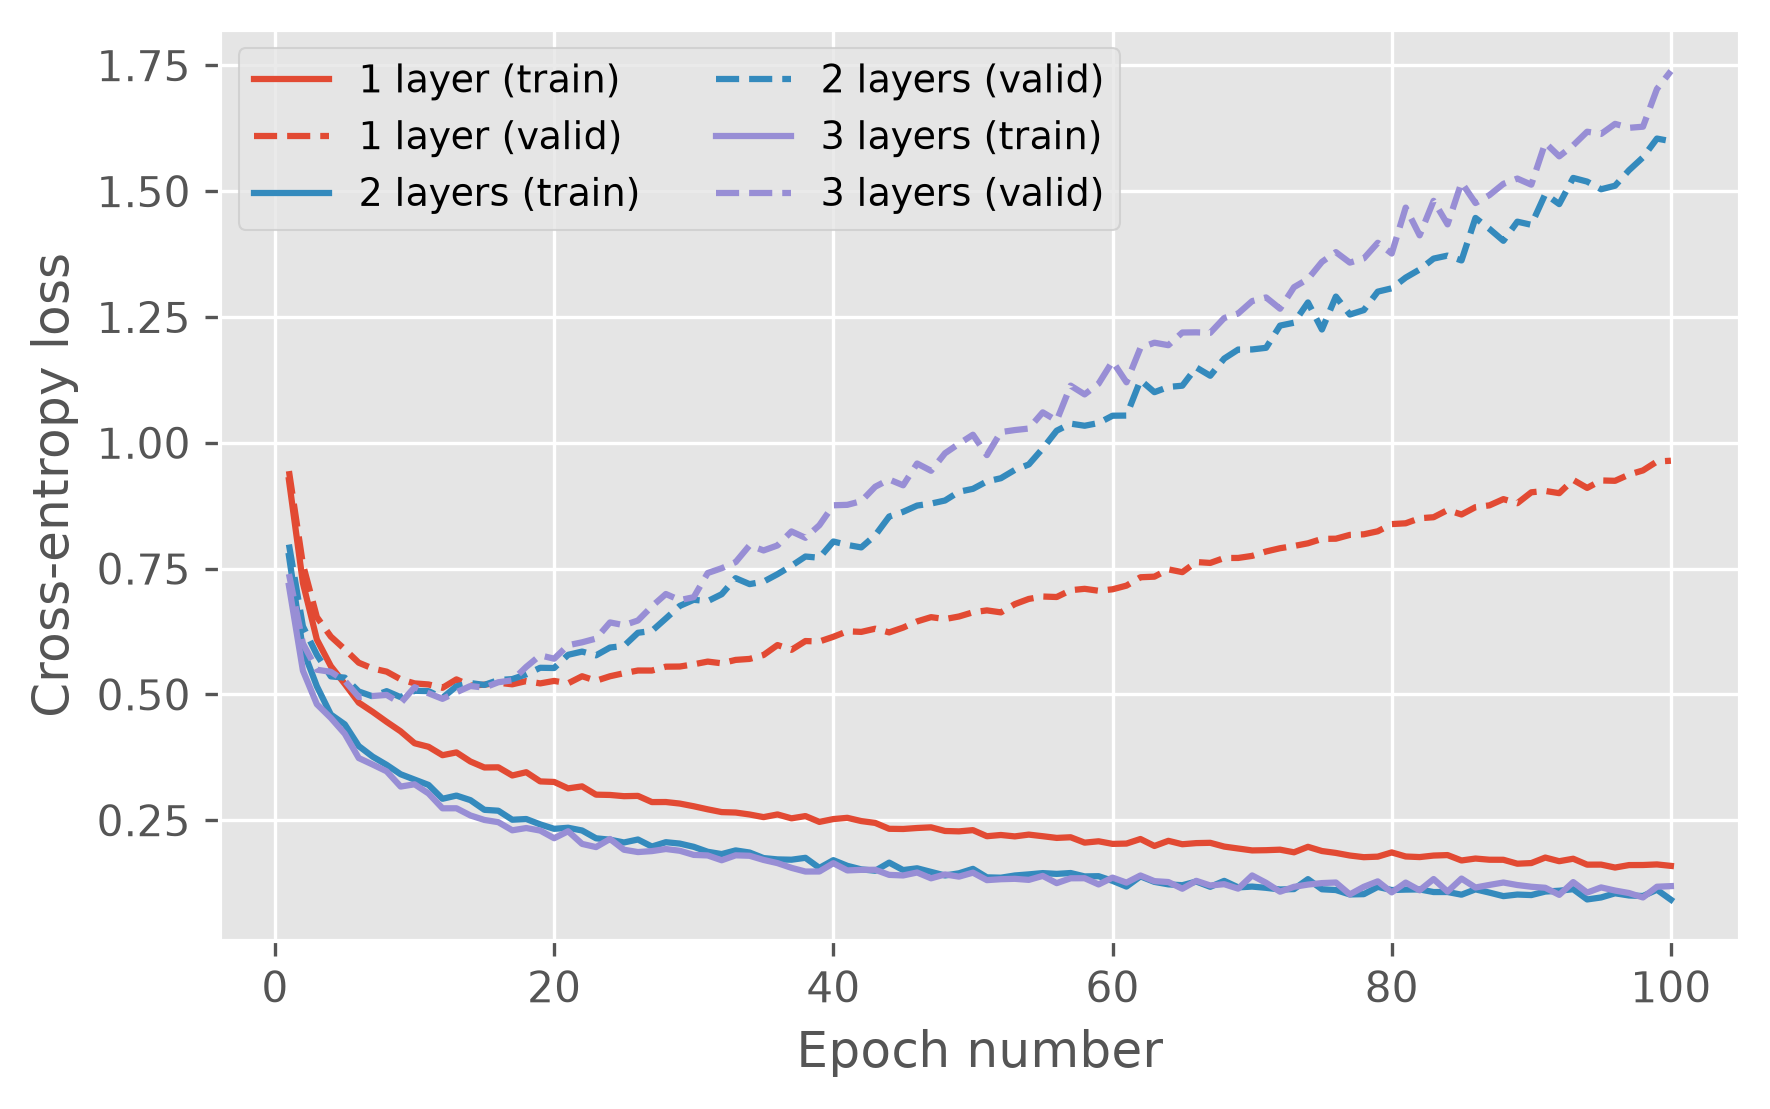
\includegraphics[width=\linewidth]{figures/fig3_depth_loss.png}
            \caption{Cross-entropy by epoch.}
            \label{fig:depth_errorcurves}
        \end{subfigure}
        \caption{Training (solid) and validation (dashed) accuracy and cross-entropy over 100 epochs for networks with one, two, or three ReLU hidden layers, each with 128 units.}
        \label{fig:depth}
    \end{figure}
}

%% Question Figure 4:
\newcommand{\questionFigureFour} {
\youranswer{Question Figure 4 - Replace these images with figures depicting the Validation Accuracy and Generalisation Gap (difference between validation and training error) for each of the experiment results varying the Dropout inclusion rate, and L1/L2 weight penalty depicted in Table 3 (including any results you have filled in).
%
\begin{figure*}[t]
    \centering
    \begin{subfigure}{.475\linewidth}
        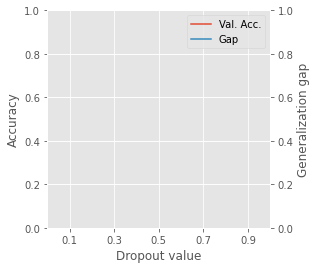
\includegraphics[width=\linewidth]{figures/empty_dropout_plot.png}
        \caption{Validation accuracy and generalisation gap by inclusion probability.}
        \label{fig:dropoutrates}
    \end{subfigure} 
    \begin{subfigure}{.475\linewidth}
        \centering
        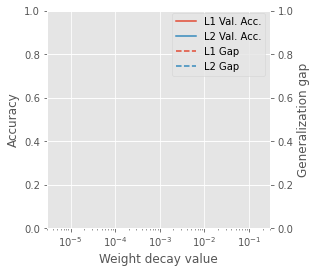
\includegraphics[width=\linewidth]{figures/empty_wd_plot.png}
        \caption{Validation accuracy and generalisation gap by penalty coefficient.}
        \label{fig:weightrates}
    \end{subfigure} 
    \caption{Epoch-100 validation accuracy and generalisation gap (validation minus training cross-entropy) against regularisation strength for dropout and L1/L2 regularisation.}
    \label{fig:hp_search}
\end{figure*}
}
}

%% Question Figure 5:
\newcommand{\questionFigureFive} {
\youranswer{Question Figure 5 - Add figures depicting the Validation Accuracy and Generalisation Gap (difference between validation and training error) for each of your 10 experiments depicted in Table 4.
}
}

%% Question Figure 6:
% \newcommand{\questionFigureSix} {
% \youranswer{Question Figure 6 - Add figures depicting the Training Accuracy, Error, and Gradient Flow Across Parameter Tensors for the one experiment run with the provided custom activation (produce these by running the "Problematic Training" cell in the Coursework\_1.ipynb notebook).
% }
% }

%% - - - - - - - - - - - - TABLES - - - - - - - - - - - - 

%% Question Table 1:
\newcommand{\questionTableOne} {
    \begin{table}[t]
        \centering
        \begin{tabular}{c|ccc}
        \toprule
        \# Hidden Units & Val. Acc. & Train Error & Val. Error \\
        \midrule
        32 & 78.9 & 0.556 & 0.694 \\
        64 & 81.1 & 0.339 & 0.665 \\
        128 & 80.7 & 0.159 & 0.964 \\
        \bottomrule
        \end{tabular}
        \caption{Epoch-100 validation accuracy (\%) and training/validation cross-entropy for one-hidden-layer ReLU networks on EMNIST.}
        \label{tab:width_exp}
    \end{table}
}

%% Question Table 2:
\newcommand{\questionTableTwo} {
    \begin{table}[t]
        \centering
        \begin{tabular}{c|ccc}
        \toprule
        \# Hidden Layers & Val. Acc. & Train Error & Val. Error \\
        \midrule
        1 & 80.7 & 0.159 & 0.964 \\
        2 & 81.5 & 0.092 & 1.599 \\
        3 & 81.8 & 0.119 & 1.739 \\
        \bottomrule
        \end{tabular}
        \caption{Epoch-100 validation accuracy (\%) and training/validation cross-entropy for ReLU networks with 128 units per hidden layer on EMNIST. Adam learning rate $10^{-3}$, batch size 100, seed 111020.}
        \label{tab:depth_exps}
    \end{table}
}

%% Question Table 3:
\newcommand{\questionTableThree} {
\youranswer{
Question Table 3 - Fill in Table 3 with the results from your experiments for the missing hyperparameter values for each of L1 regularisation, L2 regularisation, Dropout and label smoothing (use the values shown on the table). For Na\"ive Elastic Net, you need to implement the technique, choose an appropriate set of hyperparameter values, and report the results of one experiment in the table.
%
\begin{table*}[t]
    \centering
    \begin{tabular}{c|c|ccc}
    \toprule
        Model    &  Hyperparameter value(s) & Validation accuracy (\%) & Train Error & Validation Error \\
    \midrule
    \midrule
        Baseline &  -                    & 84.0 & 0.242 & 0.530 \\
    \midrule
        \multirow{4}*{Dropout}
                 & 0.6                   & 81.7 & 0.487 & 0.551 \\
                 & 0.7 & --.- & -.--- & -.---  \\
                 & 0.85 & 85.2 & 0.305 & 0.429 \\
                 & 0.97 & 85.6 & 0.229 & 0.447 \\
    \midrule
        \multirow{4}*{L1 penalty}
                 & 5e-4 & 79.6 & 0.643 & 0.663 \\
                 & 1e-3 & --.- & -.--- & -.--- \\
                 & 5e-3 & 2.19 & 3.850 & 3.850 \\
                 & 5e-2 & 2.13 & 3.850 & 3.850 \\
    \midrule
        \multirow{4}*{L2 penalty}  
                 & 5e-4 & 84.6 & 0.312 & 0.460 \\
                 & 1e-3 & --.- & -.--- & -.--- \\
                 & 5e-3 & 81.7 & 0.579 & 0.601 \\
                 & 5e-2 & 44.2 & 2.117 & 2.118 \\
    \midrule
        Label smoothing & 0.1 & --.- & -.--- & -.--- \\
    \midrule
        Na\"ive Elastic Net & --.- & --.- & -.--- & -.--- \\
    \bottomrule
    \end{tabular}
    \caption{Results of the individual-method experiments.
Report epoch-100 results, matching the supplied entries,
with random seed 111020. Errors are ordinary cross-entropy
against the original, unsmoothed labels and exclude all
weight penalties. \emph{Italics} indicate the best configuration
for each method (dropout, L1 regularisation, L2 regularisation,
label smoothing and na\"ive elastic net), and \textbf{bold}
indicates the best configuration in this table. Rank
configurations by validation accuracy, using validation
cross-entropy to break ties.}
    \label{tab:hp_search}
\end{table*}
}
}


%% Question Table 4:
\newcommand{\questionTableFour} {
\youranswer{
Question Table 4 - Add a table with the results from your 10 experiments (by which we mean: 10 training runs, NOT 10 sets of experiments) varying different hyper-parameters and regularization combinations.
}
}

%% END of YOUR ANSWERS

%% END of YOUR ANSWERS



%% Do not change anything in this file. Add your answers to mlp-cw1-questions.tex



\begin{document} 

\twocolumn[
\mlptitle{MLP 2026/27: Coursework 1}
\centerline{\studentNumber}
\vskip 7mm
]


\begin{abstract} 
This report investigates overfitting in feedforward neural networks
on the EMNIST Balanced dataset. We begin with supplied analyses
of training and validation behaviour and the effects of network
width and depth. We then examine dropout, L1 and L2 weight
penalties, na\"ive elastic net and label smoothing. Using supplied
results and additional experiments, we compare their effects on
validation performance and the generalisation gap, and justify
and evaluate ten further configurations. We select the best
configuration from Tables~3 and~4 using validation results and
evaluate it on the test set. We also independently investigate
an additional regularisation approach from the literature,
comparing its validation results with those of the selected
configuration. Finally, we discuss the findings, limitations
and future directions.

(Please note that a normal Abstract would precisely state what those conclusions were).
\end{abstract} 


\section{Introduction}
\label{sec:intro}

This report investigates overfitting, which is the training regime where performances increase on the training set but decrease on unseen data, \footnote{Technically, overtraining is the act of training beyond a point at which performance degrades; while overfitting is training to the extent that the learnt function is more complex than required to capture the training data. They correlate, but they are not, strictly speaking, the same thing. To keep things simple, and according to common usage of the terms, we are using them interchangeably in this document, and referring to their joint effect.} in feedforward neural
networks trained on EMNIST Balanced, which contains 131,600
images of handwritten characters and digits from 47 classes,
each of size $28 \times 28$.

Section~\ref{sec:task1} presents the supplied analysis identifying
overfitting and examining the effects of network width and depth
on generalisation performance and the generalisation gap
(see Ch.~5 in \citealt{Goodfellow-et-al-2016}).

Section~\ref{sec:task2.1} describes dropout
\cite{srivastava2014dropout}, L1 and L2 weight penalties
(see Section~7.1 in \citealt{Goodfellow-et-al-2016}),
na\"ive elastic net and label smoothing.

In Section~\ref{sec:task2.2}, we evaluate these methods using
a network with three hidden layers, each containing 128
units.\footnote{We denote all layers as hidden except the
final (output) one. The depth of a network is therefore
its number of hidden layers plus one.}
We combine supplied results with five individual-method
experiments and ten additional configurations selected
and justified before running them. We compare validation
performance and generalisation gaps, select the best
configuration from Tables~3 and~4 using validation results,
and evaluate it on the test set.

We also independently identify and implement a further
regularisation approach from the literature, evaluate it
in one additional training run, and compare its validation
results with those of the selected configuration.

Section~\ref{sec:concl} draws conclusions across both
investigations, relates them to the literature, and
identifies limitations and future directions.


(Please note that a normal Introduction would precisely state what those conclusions were).

\section{Problem identification}
\label{sec:task1}

\begin{figure}[t]
    \centering
    \begin{subfigure}{\linewidth}
        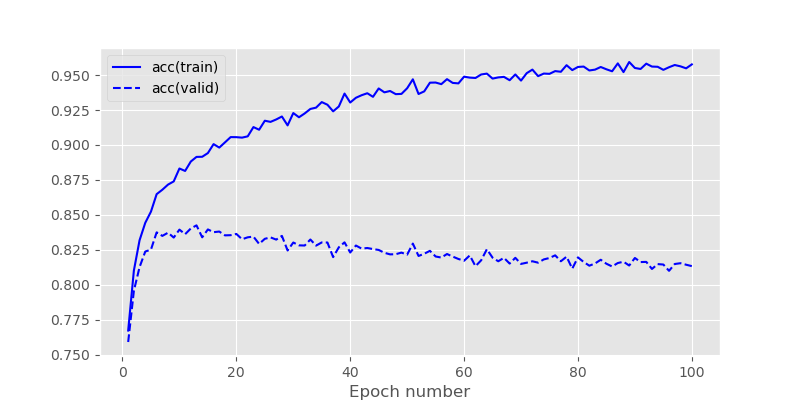
\includegraphics[width=\linewidth]{figures/fig1_acc.png}
        \caption{accuracy by epoch}
        \label{fig:example_acccurves}
    \end{subfigure} 
    \begin{subfigure}{\linewidth}
        \centering
        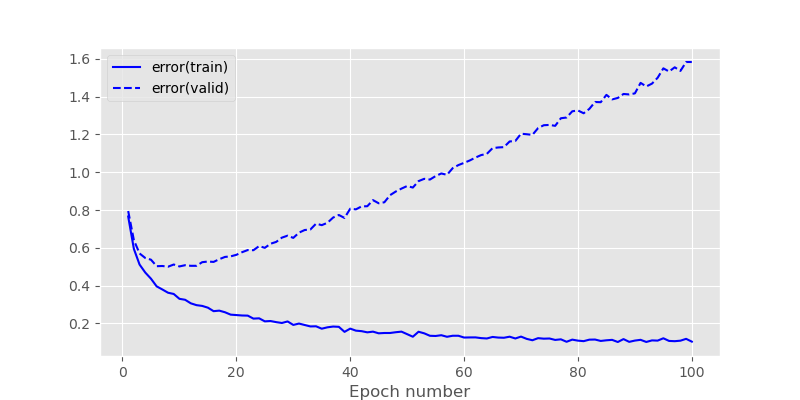
\includegraphics[width=\linewidth]{figures/fig1_err.png}
        \caption{error by epoch}
        \label{fig:example_errorcurves}
    \end{subfigure} 
    \caption{Training and validation curves in terms of classification accuracy (a) and cross-entropy error (b) on the EMNIST dataset for the baseline model.}
    \label{fig:example}
\end{figure} 

Overfitting to training data is a very common and important issue that needs to be dealt with when training neural networks or other machine learning models in general (see Ch.~5 in \citealt{Goodfellow-et-al-2016}).
A model is said to be overfitting when as the training progresses, its performance on the training data keeps improving, while its is degrading on validation data. 
Effectively, the model stops learning related patterns for the task and instead starts to memorize specificities of each training sample that are irrelevant to new samples. 
Overfitting leads to bad generalization performance in unseen data, as performance on validation data is indicative of performance on test data and (to an extent) during deployment.

Overfitting can arise when a model has too much capacity relative to the amount and diversity of training data. The more free parameters the model has, the easier it can be to fit patterns that only apply to a restricted set of training samples.
A prominent symptom of overfitting is the generalization gap, defined as the difference between the validation and training error. 
A steady increase in this quantity is usually interpreted as the model entering the overfitting regime.


Figures~\ref{fig:example_acccurves} and~\ref{fig:example_errorcurves} show the training and validation accuracy and cross-entropy error at each epoch for the baseline model.
Initially, both accuracy curves rise rapidly and both error curves fall rapidly, indicating that learning improves performance on both sets.
The training accuracy subsequently continues to increase, but at a slower rate, reaching approximately $96\%$ by the end of training.
The validation accuracy instead reaches a maximum of approximately $84\%$ around epochs 10--15, then fluctuates with a gradual downward trend towards $81\%$.
Its slope therefore changes from strongly positive to approximately zero and then slightly negative, while the training accuracy retains an overall positive slope.

The error curves make the divergence clearer.
Training error continues to decrease towards approximately $0.1$, with the rate of improvement becoming smaller as training progresses.
Validation error reaches a minimum of approximately $0.5$ around epoch 10, after which its slope becomes positive and it rises towards $1.6$.
The widening gap between falling training error and rising validation error indicates that further training is improving the fit to the training set while harming generalisation.
We therefore identify the onset of overfitting at approximately epoch 10.

The extent to which our model overfits depends on many factors.
For example, the quality and quantity of the training set and the complexity of the model. 
If we have sufficiently many diverse training samples, or if our model contains few hidden units, it will in general be less prone to overfitting. 
Appropriate regularization can also limit the extent to which the model overfits.


\subsection{Network width}

\questionTableOne
\questionFigureTwo

First we investigate the effect of increasing the number of hidden units in a single hidden layer network when training on the EMNIST dataset.
The PyTorch network is trained using the Adam optimizer
with a learning rate of $10^{-3}$ and a batch size of 100, for a total of 100 epochs.

The input layer is of size 784, and output layer consists of 47 units. 
Three different models were trained, with a single hidden layer of 32, 64 and 128 ReLU hidden units respectively.
Figure~\ref{fig:width} depicts the error and accuracy curves over 100 epochs for the model with varying number of hidden units.
Table~\ref{tab:width_exp} reports the final accuracy, training error, and validation error.

The solid curves in Figure~\ref{fig:width} show training performance, and the dashed curves show validation performance.
Increasing the width improves the fit to the training data: the epoch-100 training error decreases from $0.556$ with 32 units to $0.339$ with 64 units and $0.159$ with 128 units, while training accuracy increases.
The validation results do not follow the same monotonic trend.
Final validation accuracy is $78.9\%$, $81.1\%$, and $80.7\%$, respectively, and the corresponding validation errors are $0.694$, $0.665$, and $0.964$.
The 64-unit model therefore achieves both the highest final validation accuracy and the lowest final validation error in this series.

The curves also show that the larger models begin to overfit earlier and more strongly.
For 128 units, validation error reaches its minimum around epochs 15--20 and then increases substantially, while training error continues to decrease.
The 64-unit validation error reaches a broader minimum around epochs 25--35 and increases more slowly thereafter.
For 32 units, validation error largely flattens in the later epochs, and the separation from training error remains much smaller.
Using the rounded values in Table~\ref{tab:width_exp}, the final generalisation gaps are $0.138$, $0.326$, and $0.805$ for 32, 64, and 128 units, respectively.

These results show a consistent increase in training fit and generalisation gap as width grows, but not a consistent improvement in validation performance.
This is compatible with the capacity argument in Section~5.2 of \citet{Goodfellow-et-al-2016}: additional hidden units give the network greater flexibility to represent useful patterns, but also to fit details specific to the training set.
The relatively high training error and low accuracy of the 32-unit model suggest that its capacity constrains the fit under this training setup.
Increasing to 64 units improves validation performance, whereas increasing further to 128 units only improves training performance but produces stronger overfitting,thus bringing no improvements to the validation accuracy.


\subsection{Network depth}

\questionTableTwo
\questionFigureThree

Next we investigate the effect of varying the number of hidden layers in the network. 
Table~\ref{tab:depth_exps} and Figure~\ref{fig:depth} depict results from training three models with one, two and three hidden layers respectively, each with 128 ReLU hidden units. 
As with previous experiments, they are trained with \texttt{torch.optim.Adam} with a learning rate of $10^{-3}$ and a batch size of 100. 

Figure~\ref{fig:depth} shows that all three networks initially improve on both the training and validation sets.
The two- and three-hidden-layer models then achieve higher training accuracy than the one-hidden-layer model, reaching approximately $96\%$ rather than $94\%$ near the end of training.
Their validation errors reach minima around epoch 10 and then increase, while the one-hidden-layer model turns upwards later, around epochs 15--20.
After these turning points, validation accuracy generally declines even as training accuracy continues to improve, indicating overfitting in all three models.

Table~\ref{tab:depth_exps} quantifies the final results.
Validation accuracy increases modestly from $80.7\%$ with one hidden layer to $81.5\%$ with two and $81.8\%$ with three.
Validation error, however, increases from $0.964$ to $1.599$ and $1.739$, respectively.
The training errors are $0.159$, $0.092$, and $0.119$, giving final generalisation gaps of $0.805$, $1.507$, and $1.620$.
Thus, the three-hidden-layer model has the highest final validation accuracy but also the largest error gap, while the one-hidden-layer model has the lowest final validation error and the smallest gap.

From these results, we can conclude that both deeper networks fit the training set better than the one-hidden-layer network, but at the same time it  consistently enlarges the final generalisation gap.
As discussed in Section~6.4 of \citet{Goodfellow-et-al-2016}, the reason for these is likely due to additional layers compose nonlinear transformations and can represent more complex functions, creating a better fit to the training data, but hurting the generalizability of the model.
Even though there was a modest gain in validation accuracy with more network layers, this comes at the cost of a much larger increase in validation error, so increasing depth alone does not resolve the overfitting problem.


\section{Regularization}
\label{sec:task2.1} 

This section describes five regularisation methods:
dropout, L1 and L2 weight penalties, na\"ive elastic net
and label smoothing.


\subsection{Dropout}

Dropout~\cite{srivastava2014dropout} is a stochastic method that randomly inactivates neurons in a neural network according to an hyperparameter, the inclusion rate  (\textit{i.e.} the rate that an unit is included).
Dropout is commonly represented by an additional layer inserted between the linear layer and activation function.
Its forward pass during training is defined as follows:
\begin{align}
    \text{mask} &\sim \text{bernoulli}(q)\\
    \bm{y}' &= \frac{\text{mask} \odot \bm{y}}{q}
\end{align}
where $\bm{y}, \bm{y}' \in \mathbb{R}^d$ are the output of the linear layer before and after applying dropout, respectively. 
$\text{mask} \in \mathbb{R}^d$ is a mask vector randomly sampled from the Bernoulli distribution with inclusion probability $q$, and $\odot$ denotes the element-wise multiplication.

At inference time, stochasticity is not desired, so no neurons are dropped. 
Because PyTorch scales retained activations during training, the evaluation transformation is the identity:
\begin{align}
    \bm{y}' &= \bm{y}
\end{align}

As there is no nonlinear calculation involved, the backward propagation during training is the element-wise product of the gradients with the scaled mask; during evaluation it is unchanged. 
The backward propagation for dropout is therefore formulated as follows:
\begin{align}
    \frac{\partial \bm{y}'}{\partial \bm{y}} = \frac{mask}{q}
\end{align}

Dropout is an easy to implement and highly scalable method. 
It can be implemented as a layer-based calculation unit, and be placed on any layer of the neural network at will. 
Dropout can reduce the dependence of hidden units between layers so that the neurons of the next layer will not rely on only few features from of the previous layer.
Instead, it forces the network to extract diverse features and evenly distribute information among all features. 
By randomly dropping some neurons in training, dropout makes use of a subset of the whole architecture, so it can also be viewed as bagging different sub networks and averaging their outputs.


\subsection{Weight penalty}

L1 and L2 regularization~\cite{ng2004feature} are simple but effective methods to mitigate overfitting to training data. 
The application of L1 and L2 regularization strategies could be formulated as adding penalty terms with L1 and L2 norm square of weights in the cost function without changing other formulations. 
The idea behind this regularization method is to penalize the weights by adding a term to the cost function, and explicitly constrain the magnitude of the weights with either the L1 and L2 norms.
The optimization problem takes a different form:
\begin{align}
    \text{L1: } & \text{min}_{\bm{\theta}} \; E_{\text{data}}(\bm{X}, \bm{y}, \bm{\theta}) + \lambda_1 \sum_i|\theta_i|\\
    \text{L2: } & \text{min}_{\bm{\theta}} \; E_{\text{data}}(\bm{X}, \bm{y}, \bm{\theta}) + \frac{\lambda_2}{2}\sum_i\theta_i^2
\end{align}
where $E_{\text{data}}$ denotes the cross-entropy loss on the model logits, $\{\bm{X}, \bm{y}\}$ denotes the input and target training pairs, and $\bm{\theta}$ includes the trainable weights and biases. 
$\lambda_1$ and $\lambda_2$ control the strengths of the two regularizers.

Weight penalty works by constraining the scale of parameters and preventing them to grow too much, avoiding overly sensitive behaviour on unseen data.
While L1 and L2 regularization are similar to each other in calculation, they have different effects.
Gradient magnitude in L1 regularization does not depend on the weight value and tends to bring small weights to 0, which can be used as a form of feature selection, whereas L2 regularization tends to shrink the weights to a smaller scale uniformly. 

\subsubsection{Na\"ive Elastic Net Regularisation}

\questionOne.

\subsection{Label smoothing}
Label smoothing regularizes a model based on a softmax with $K$ output values. PyTorch's $\texttt{label\_smoothing}$ parameter inside $\texttt{torch.nn.CrossEntropyLoss()}$  mixes each one-hot target with the uniform distribution:
\begin{equation}
    t'_k=(1-\alpha)t_k+\frac{\alpha}{K}.
\end{equation}
Here $\alpha$ is typically set to a small number such as $0.1$. The criterion receives logits and integer targets, and applies this smoothing only when computing the training loss.
This strategy may prevent a neural network to obtain very large weights by discouraging very high output values.

\section{Balanced EMNIST Experiments}

\questionTableThree

\questionFigureFour

\questionTableFour

\questionFigureFive

% \questionFigureSix

\label{sec:task2.2}

Here we evaluate regularisation methods on EMNIST Balanced.
The common architecture has three hidden layers, each with
128 units. The prescribed experiments use a learning rate
of $10^{-4}$ and the other common settings specified in
the coursework description.

Table~\ref{tab:hp_search} combines supplied results with
five required training runs: one each for dropout, L1,
L2, label smoothing and na\"ive elastic net. For dropout,
L1, L2 and label smoothing, we use the specified
hyperparameter values. For na\"ive elastic net, we choose
and justify the hyperparameter values.

Figure~\ref{fig:hp_search} plots epoch-100 validation
accuracy and generalisation gap against regularisation
strength for dropout, L1 and L2.

Using these results, we select and justify ten additional
configurations before running them, and present their
results in Table~4 and Figure~5. We analyse the prescribed
experiments and select and test the best configuration
from Tables~3 and~4 in Question~4.

Question~5 presents an independent regularisation
investigation comprising one additional training run,
with its validation results compared against those of
the configuration selected in Question~4.

\questionTwo.

\questionThree.

% \subsection{Custom Activation Function}

\questionFour.

\questionFive.

\section{Conclusion}
\label{sec:concl}
    
\questionSix.

\newpage
\bibliography{ref}

\end{document} 
